\documentclass[12pt]{article}

% -----------------------------------------------
% PACOTES OBRIGATÓRIOS (SBC TEMPLATE OFICIAL)
% -----------------------------------------------
\usepackage{sbc-template}           % Estilo oficial SBC — inclui geometry, times, caption e sections
\usepackage{graphicx,url}
\usepackage[T1]{fontenc}
\usepackage[utf8]{inputenc}
\usepackage[brazil,english]{babel}

% Pacotes complementares (não conflitam com sbc-template)
\usepackage{enumitem}
\setlist[itemize]{label=--}
\usepackage{booktabs}
\usepackage{tikz}
\usetikzlibrary{shapes.geometric,arrows.meta,positioning,fit,backgrounds}

\sloppy

% -----------------------------------------------
% CABEÇALHO
% -----------------------------------------------
\title{Medição Automatizada de QoE e UX Sustentável com Playwright:\\
       Um Instrumento para Redução de Desperdício Computacional na Web}

\author{Mariana Ribeiro\inst{1}, Vinícius Schineider Januário Viana\inst{1},\\
        Simone Azevedo Bandeira de Melo Aquino\inst{1}}

\address{Instituto Federal de Educação, Ciência e Tecnologia do Maranhão (IFMA) -- Campus Imperatriz\\
  Imperatriz -- MA -- Brasil
  \email{\{mariana.r,viniciusschineider\}@acad.ifma.edu.br,
  simonebandeira@ifma.edu.br}
}

\begin{document}

\maketitle

% -----------------------------------------------
% RESUMOS — sbc-template.sty insere "Abstract."
% e "Resumo." automaticamente em itálico negrito;
% NÃO repetir o prefixo aqui.
% -----------------------------------------------
\begin{abstract}
Web UX evaluation typically relies on post-hoc subjective methods, which are
unable to capture latent friction occurring during interaction. This paper
proposes and validates a Playwright-based instrument for automated Quality of
Experience (QoE) measurement, operating as a passive listener that
unobtrusively captures behavioral metrics --- dead clicks and long hesitations
--- as proxies for interface friction and computational waste. A mixed-methods
controlled study was conducted with 9 participants on the DevShare platform,
covering four interaction flows. Objective metrics were cross-validated with
UEQ-S subjective scores and open-ended qualitative responses. Thematic
analysis revealed that 78\% of participants spontaneously reported absence of
visual feedback, the exact behavior captured by the instrument via dead click
detection. Although Spearman correlation between friction score and UEQ-S
pragmatic quality did not reach significance ($\rho = +0.13$, $p = 0.73$,
$N = 9$) --- consistent with a power analysis indicating $N \geq 30$ for
confirmatory results --- the qualitative triangulation confirms the
instrument's construct validity. The findings position automated behavioral
monitoring as a complementary approach to subjective evaluation, with
implications for Sustainable UX and Green Software Engineering.
\end{abstract}

\begin{resumo}
A avaliação de UX web tipicamente recorre a métodos subjetivos post-hoc,
incapazes de capturar o atrito latente durante a interação. Este artigo propõe
e valida um instrumento baseado em Playwright para medição automatizada de
Qualidade de Experiência (QoE), atuando como observador passivo não intrusivo
que registra métricas comportamentais --- \textit{dead clicks} e hesitações
prolongadas --- como \textit{proxies} de atrito de interface e desperdício
computacional. Um estudo controlado de métodos mistos foi conduzido com 9
participantes na plataforma DevShare, cobrindo quatro fluxos de interação. As
métricas objetivas foram validadas cruzadamente com scores UEQ-S e respostas
qualitativas abertas. A análise temática revelou que 78\% dos participantes
relataram espontaneamente ausência de \textit{feedback} visual --- exatamente
o comportamento capturado pelo instrumento via detecção de \textit{dead
clicks}. Embora a correlação de Spearman entre o \textit{friction score} e a
qualidade pragmática UEQ-S não tenha atingido significância ($\rho = +0{,}13$,
$p = 0{,}73$, $N = 9$) --- consistente com análise de poder indicando
$N \geq 30$ para resultados confirmatórios --- a triangulação qualitativa
confirma a validade de construto do instrumento. Os achados posicionam o
monitoramento comportamental automatizado como abordagem complementar à
avaliação subjetiva, com implicações para UX Sustentável e Green Software.
\end{resumo}

% ==========================================
% CORPO DO ARTIGO
% ==========================================
\section{Introdução}

A avaliação da Qualidade de Experiência (QoE) e da Usabilidade (UX) em aplicações Web tem sido, historicamente, conduzida por meio de métodos manuais e subjetivos. Os métodos atuais dependem majoritariamente de intervenções aplicadas a posteriori ou de práticas de \textit{Quality Assurance} (QA) focadas na validação sintética de regressões funcionais [Leppänen 2024]. No entanto, a lacuna metodológica na automação de testes reside na distinção clássica entre sintaxe e semântica: algoritmos podem validar códigos sem possuir intencionalidade ou compreensão sobre a frustração emocional vivenciada durante a interação [Searle 1982, Rousi 2019].

Além do aspecto humano, a ineficiência no design de interfaces configura-se como um vetor de desperdício de recursos. Gargalos de usabilidade induzem os usuários a comportamentos erráticos --- como cliques repetidos (\textit{dead clicks}) e hesitações prolongadas. No contexto de aplicações Web, essas interações desencadeiam cascatas de requisições HTTP desnecessárias, atuando como indicadores de sobrecarga computacional e pegada de carbono, o que a literatura recente classifica como antipadrões de energia web [Oyedeji et al. 2019, Rani et al. 2024].

Para endereçar este problema, este artigo propõe o desenvolvimento de um instrumento automatizado que integra a avaliação de Interação Humano-Computador (IHC) com premissas de Engenharia de Software Sustentável (Green IT). O trabalho altera a aplicação convencional do framework \textit{Playwright}: em vez de executar rotinas sintéticas de clique, a ferramenta atua como observador passivo da jornada de usuários reais, capturando rastros de telemetria sem instrumentação intrusiva.

O presente artigo detalha a arquitetura desta solução e apresenta um desenho experimental estruturado na plataforma Web ``DevShare''. O estudo busca correlacionar os \textit{logs} automatizados com a percepção subjetiva reportada via questionário UEQ-S. O objetivo é investigar como a volumetria de dados sintáticos capturados pela máquina [Rousi 2019] pode atuar como uma auditoria contínua de UX sustentável.

\section{Fundamentação Teórica e Trabalhos Relacionados}

O instrumento proposto fundamenta-se na intersecção entre a filosofia da percepção, a automação de medição de QoE e as premissas de eficiência de recursos (\textit{Green UX}).

\textbf{Sintaxe, Semântica e Metas de UX:} A experiência do usuário divide-se fundamentalmente em metas pragmáticas e hedônicas [Grigis e De Angeli 2024], cujas barreiras são sintetizadas na Tabela 1.

\begin{table}[htbp]
  \centering
  \caption{Diretores e barreiras em função das metas de UX}
  \begin{tabular}{p{2.5cm} p{4cm} p{7cm}}
    \toprule
    \textbf{Metas de UX} & \textbf{Diretores (Drivers)} & \textbf{Barreiras (Barriers)} \\
    \midrule
    \textbf{Pragmáticas} & Utilidade & Limitações técnicas, disponibilidade, perda econômica \\
    \textbf{Hedônicas} & Surpresa, fascinação & Ameaça à identidade, política (filtros e tabus) \\
    \bottomrule
  \end{tabular}
\end{table}

Ferramentas clássicas de QA atuam prioritariamente sobre barreiras pragmáticas. Conforme o experimento mental do ``Quarto Chinês'' [Searle 1982], um script de automação manipula a interface corretamente através de regras pré-definidas, mas carece de agência para interpretar a degradação da experiência. Sem o acompanhamento empírico humano, os logs automatizados tendem a atuar como ``significantes vazios'' [Rousi 2019]. A abordagem aqui proposta delega à máquina (Playwright) exclusivamente a captura da \textit{sintaxe} das interações em tempo real (tempos e eventos), condicionando a interpretação \textit{semântica} ao cruzamento com dados humanos (UEQ-S).

\textbf{Automação Passiva e UX Sustentável:} Estudos sustentam a viabilidade de afastar a dependência exclusiva da subjetividade humana em avaliações. No cenário nacional, Garcia et al. (2023) já apontavam a necessidade de estruturas para a automatização do diagnóstico de UX, destacando a urgência de métricas quantitativas. Internacionalmente, Keshvadi e Williamson (2020) empregaram a ferramenta MoVIE para capturar tráfego passivamente e inferir QoE, enquanto Banaouas (2019) evidenciou que 55\% das heurísticas de usabilidade podem ser diagnosticadas via sequenciamento de eventos de GUI.

A contribuição da presente pesquisa concentra-se em conectar essa automação empírica ao domínio de \textit{Green Software}. A avaliação energética do software é reconhecida como uma contribuição essencial para a Computação Verde [Autores SBSI 2013], figurando como fator competitivo no mercado de TI [Autores WSIS].

Para viabilizar esta ligação, Teixeira e Fook (2025) mapearam requisitos não-funcionais para software sustentável, ao passo que Oyedeji et al. (2019) e Rani et al. (2024) documentaram a interação entre usabilidade e aspectos verdes. A premissa adotada é que a eliminação de atritos de interface previne ações repetitivas, que se traduziriam em processamento redundante. Neste contexto, rastrear falhas de usabilidade via ferramentas de escuta passiva --- estruturalmente mais leves que automações baseadas em processamento de imagens, como o Sikuli [Savoldi e Oliveira 2018] --- constitui uma tática de prevenção de ineficiência de código.

\section{Metodologia e Arquitetura do Instrumento}

A pesquisa caracteriza-se como um estudo metodológico e uma Prova de Conceito (PoC), operacionalizada por meio de um desenho quase-experimental controlado. O objetivo é verificar a correlação empírica entre falhas de interface (sintaxe), percepção do usuário (semântica) e volume de dados trafegados (proxy de desperdício).

\subsection{O Playwright como Auditor Passivo no CI/CD}

A principal característica da arquitetura proposta é a instanciação do \textit{Playwright} em modo \textit{listen-only} (escuta). Idealizado para ser acoplado ao pipeline de homologação (CI/CD), a ferramenta injeta um script ouvinte via API \texttt{page.addInitScript}, interceptando eventos customizados \texttt{qoe:step} no \textit{front-end}. O sistema monitora três indicativos:

\begin{itemize}
    \item \textbf{Duração do Fluxo:} Tempo total de atividade para conclusão da tarefa;
    \item \textbf{Dead Clicks:} Cliques sem resposta perceptível do sistema, capturados via instrumentação de eventos DOM, que evidenciam interações mal-sucedidas do usuário;
    \item \textbf{Hesitação:} Períodos de inatividade superiores a 10 segundos entre transições de página, limiar definido a partir da literatura de tempos de resposta aceitáveis em interfaces Web [Nielsen 1994], sugerindo desorientação ou sobrecarga cognitiva.
\end{itemize}

Esta arquitetura viabiliza uma coleta não intrusiva, dispensando a inserção de bibliotecas de telemetria de terceiros no código de produção.\footnote{Artefatos do estudo (código-fonte, dados anonimizados e scripts de análise) disponíveis em: \texttt{[URL\_ANONIMA]}.}

\begin{figure}[htbp]
\centering
\begin{tikzpicture}[
  font=\small,
  box/.style={rectangle, draw, rounded corners=3pt, minimum width=2.2cm,
              minimum height=0.9cm, align=center, fill=white},
  grp/.style={rectangle, draw=gray!60, rounded corners=4pt,
              inner sep=6pt, fill=gray!8},
  arr/.style={-{Stealth[length=5pt]}, thick},
  lbl/.style={font=\tiny, midway, above, sloped}
]

% --- Nós ---
\node[box] (user) {Usuário\\(participante)};

% Grupo: DevShare
\node[box, right=1.1cm of user]  (iface)  {Interface\\React/Next.js};
\node[box, below=0.5cm of iface] (event)  {\texttt{qoe:step}\\dispatcher};
\begin{scope}[on background layer]
  \node[grp, fit=(iface)(event), label={[font=\footnotesize]above:DevShare · localhost}] (fe) {};
\end{scope}

% Grupo: Playwright
\node[box, right=1.1cm of iface]  (init)    {\texttt{addInitScript}\\(ouvinte)};
\node[box, below=0.5cm of init]   (capture) {Captura DOM\\+ timestamps};
\begin{scope}[on background layer]
  \node[grp, fit=(init)(capture), label={[font=\footnotesize]above:Playwright · listen-only}] (pw) {};
\end{scope}

% Grupo: Saída
\node[box, right=1.1cm of init]   (dc)   {\textit{dead clicks}};
\node[box, below=0.25cm of dc]    (hes)  {hesitações $\geq$10\,s};
\node[box, below=0.25cm of hes]   (dur)  {duração do fluxo};
\begin{scope}[on background layer]
  \node[grp, fit=(dc)(hes)(dur), label={[font=\footnotesize]above:Saída · CSV}] (out) {};
\end{scope}

% --- Setas ---
\draw[arr] (user)    -- node[lbl]{interage} (iface);
\draw[arr] (iface)   -- (event);
\draw[arr] (event.east) -- ++(0.4,0) |- node[lbl, near end]{escutado por} (init.west);
\draw[arr] (init)    -- (capture);
\draw[arr] (capture.east) -- ++(0.4,0) |- (dc.west);
\draw[arr] (capture.east) -- ++(0.4,0) |- (hes.west);
\draw[arr] (capture.east) -- ++(0.4,0) |- (dur.west);

\end{tikzpicture}
\caption{Esquema arquitetural para auditoria passiva via Playwright. O script ouvinte é injetado via \texttt{page.addInitScript}; eventos \texttt{qoe:step} do \textit{front-end} são capturados em tempo real, sem instrumentação intrusiva no código de produção.}
\label{fig:arquitetura}
\end{figure}

\subsection{Objeto de Estudo: A Plataforma DevShare}

Os testes empregam a ``DevShare'', aplicação Web desenvolvida como artefato de pesquisa para o nicho de compartilhamento de dicas entre profissionais de tecnologia (desenvolvedores, designers e operações). Construída com Next.js (App Router) e React, sua interface é projetada para avaliações de tarefas pragmáticas e utilitárias.\footnote{Instância pública disponível em: \texttt{[URL\_VERCEL]} (SPA sem \textit{backend}; persistência em \texttt{localStorage}).}

A fim de isolar instabilidades inerentes a conexões externas de internet, a aplicação utiliza persistência em memória local (\texttt{localStorage}). Para reproduzir latências de rede sem dependência de infraestrutura externa, o código implementa \textbf{mocks assíncronos} (via \texttt{setTimeout} e resolução de promessas), que introduzem atrasos programados nas operações de escrita e leitura. O Playwright captura os efeitos comportamentais dessas latências --- hesitações e \textit{dead clicks} --- via eventos DOM e timestamps de navegação, independentemente do mecanismo subjacente de persistência. Esta escolha de design isola a variável de interesse (atrito de \textit{feedback} da interface) dos fatores de variabilidade de infraestrutura.

\subsection{Desenho Experimental e Cenários}

A execução das tarefas compreende quatro fluxos independentes, mapeados na Tabela 2. Os fluxos foram definidos para cobrir as principais jornadas pragmáticas da plataforma: exploração de conteúdo, criação de publicação, interação social e configuração de perfil.

\begin{table}[htbp]
  \centering
  \caption{Fluxos de interação definidos como unidades de análise}
  \begin{tabular}{p{2.8cm} p{2.5cm} p{2cm} p{5.2cm}}
    \toprule
    \textbf{Fluxo} & \textbf{Tipo} & \textbf{Condição} & \textbf{Característica} \\
    \midrule
    \textbf{explorar-salvar}  & Exploratório & Baseline  & Navegação livre pelo feed; maior volume de conteúdo \\
    \textbf{postar-dica}      & Criação      & Degradado & Ausência de \textit{feedback} visual após submissão do formulário \\
    \textbf{criar-perfil}     & Configuração & Degradado & Ausência de indicador de carregamento após confirmação \\
    \textbf{comentar-reagir}  & Social       & Neutro     & Interação com publicações existentes; sem degradação induzida \\
    \bottomrule
  \end{tabular}
\end{table}

Nos fluxos degradados, a supressão de \textit{feedback} de carregamento configura uma violação das heurísticas de visibilidade do estado do sistema [Nielsen 1994, Molich e Nielsen 1990], com o intuito de induzir comportamentos erráticos mensuráveis --- em especial \textit{dead clicks} e hesitações prolongadas. Os participantes executaram as tarefas sem conhecimento prévio das degradações inseridas.

\subsection{Ambiente de Teste e Protocolo de Coleta de Dados}

O experimento contemplou 9 participantes com perfil de profissionais ou estudantes de tecnologia. O desenho é \textbf{within-subjects}: cada participante executou os quatro fluxos sequencialmente, em ordem fixa, em uma única sessão. A ordem foi padronizada para controlar efeitos de aprendizado: (1) explorar-salvar, (2) postar-dica, (3) criar-perfil, (4) comentar-reagir. A coleta foi presencial, em computador controlado de laboratório, para mitigar variabilidade de hardware:

\begin{enumerate}
    \item \textbf{Briefing:} O participante recebeu o roteiro de tarefas, ciente da gravação das interações via Termo de Consentimento Livre e Esclarecido (TCLE), mas sem conhecimento das degradações experimentais.
    \item \textbf{Execução Interativa (Sintaxe):} O usuário interagiu com a plataforma servida em \texttt{localhost}. O Playwright registrou em segundo plano os logs quantitativos: timestamps de navegação, contagem de \textit{dead clicks} e duração de cada fluxo.
    \item \textbf{Avaliação Subjetiva (Semântica):} Ao fim das tarefas, o participante avaliou sua experiência por meio do \textit{User Experience Questionnaire -- Short} (UEQ-S, escala $-3$ a $+3$, 4 itens pragmáticos e 4 hedônicos) e respondeu a três perguntas abertas: (Q1) ``Houve algum momento em que você ficou confuso ou sem saber o que fazer?''; (Q2) ``Alguma ação produziu um resultado inesperado ou diferente do que você esperava?''; (Q3) ``O que você mudaria na plataforma?''.\footnote{Instrumento UEQ-S, planilha de pontuação e dados normativos: \texttt{ueq-online.org}.}
\end{enumerate}

A dissociação temporal metodológica entre a coleta mecânica (silenciosa) e o relato humano permite a estruturação de um estudo de \textbf{métodos mistos}, viabilizando a triangulação dos dados.

\section{Resultados e Discussão}

\subsection{Métricas Objetivas por Fluxo}

A Tabela 3 apresenta as métricas agregadas por fluxo para os 9 participantes. O \textit{FrictionScore} é calculado em dois estágios: (1) para cada participante, compõe-se um score de sessão ponderando \textit{dead clicks} (peso 0,4), hesitações longas $\geq 10$ s (peso 0,4) e duração total (peso 0,2), todos normalizados individualmente por min-max; (2) para comparação entre fluxos, agrega-se a média por fluxo e reaplicam-se os pesos duração (0,6) e hesitações (0,4), resultando em um índice de 0 a 100. Os pesos refletem a premissa de que eventos discretos de clique e pausas longas são sinais mais diretos de fricção do que a duração bruta, que pode ser legitimamente alta em fluxos exploratórios.

\begin{table}[htbp]
  \centering
  \caption{Métricas objetivas agregadas por fluxo ($N = 9$)}
  \begin{tabular}{p{3.2cm} r r r r r}
    \toprule
    \textbf{Fluxo} & \textbf{N} & \textbf{Dur. média (s)} & \textbf{DP (s)} & \textbf{Hesit. média} & \textbf{FrictionScore} \\
    \midrule
    explorar-salvar  & 9 & 337,8 & 222,3 & 6,20 & 100,00 \\
    criar-perfil     & 9 & 253,8 & 266,9 & 2,30 &  32,02 \\
    comentar-reagir  & 9 & 162,6 & 210,0 & 3,44 &  12,29 \\
    postar-dica      & 9 & 169,5 & 135,6 & 2,22 &   2,37 \\
    \bottomrule
  \end{tabular}
\end{table}

Dois padrões aparentemente paradoxais emergem dos dados e permitem demonstrar a capacidade discriminatória do instrumento quando seus sinais são analisados em conjunto. Primeiro, o fluxo \textit{explorar-salvar} apresentou o maior FrictionScore apesar de ser baseline. A triangulação, porém, resolve a aparente contradição: a análise temática não registrou nenhuma menção de \textit{feedback} ausente, botão sem resposta ou redirecionamento falho neste fluxo, e a contagem de \textit{dead clicks} associada a ele foi a mais baixa entre todos os fluxos. Hesitações longas sem \textit{dead clicks} e sem corroboração qualitativa negativa configuram um padrão distinto --- o de \textbf{leitura engajada}, não de fricção. Isso evidencia que, quando os dois sinais do instrumento (comportamento temporal e eventos discretos de clique) divergem e o qualitativo confirma a ausência de frustração, a hesitação deve ser interpretada como cognitivamente positiva. Segundo, o fluxo \textit{postar-dica}, intencionalmente degradado, apresentou o menor score de duração --- mas não o menor índice de fricção real. Os \textit{dead clicks} registrados neste fluxo, associados ao tema qualitativo ``botão sem resposta perceptível'' (33\% dos participantes), confirmam que a fricção ocorreu mesmo quando a duração bruta foi reduzida pelo comportamento de abandono precoce de parte dos participantes. A discrepância entre duração curta e frustração verbalizada é ela própria um achado: \textbf{sessões curtas em fluxos degradados indicam desistência, não fluência} --- distinção que o \textit{dead click} captura e a duração isolada não captura. Esses dois casos demonstram que a validade diagnóstica do instrumento emerge da leitura cruzada de seus componentes, não de qualquer métrica isolada.

Em nível de sessão, registraram-se 44 \textit{dead clicks} totais entre os 9 participantes (média: 4,9; máximo: 29, por P04), com duração média de sessão de 478,7 s (mín: 235,9 s; máx: 1011,7 s).

\begin{figure}[htbp]
  \centering
  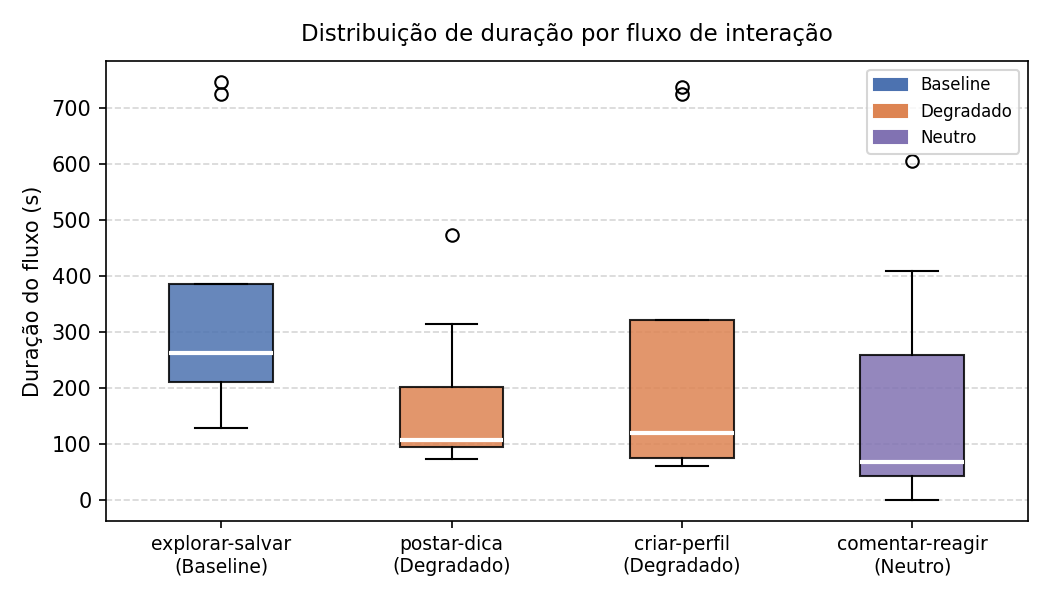
\includegraphics[width=0.92\linewidth]{plots/flow_duration_boxplot.png}
  \caption{Distribuição da duração por fluxo (boxplot, $N = 9$). A amplitude interquartil ampla do fluxo \textit{explorar-salvar} reflete a heterogeneidade de ritmo de leitura entre participantes; o menor desvio de \textit{postar-dica} reflete a uniformidade do comportamento de abandono prematuro.}
  \label{fig:boxplot}
\end{figure}

\subsection{Análise Temática das Respostas Qualitativas}

As respostas abertas (Q1--Q3) foram submetidas a \textbf{análise de conteúdo com categorização dedutiva} [Bardin 1977]: categorias temáticas foram definidas \textit{a priori} a partir das heurísticas de Nielsen (1994) e dos mecanismos de captura do instrumento, e as respostas foram classificadas por busca de palavras-chave e expressões associadas a cada categoria. A Figura~\ref{fig:temas} e a Tabela 4 apresentam a frequência de cada categoria detectada.

\begin{figure}[htbp]
  \centering
  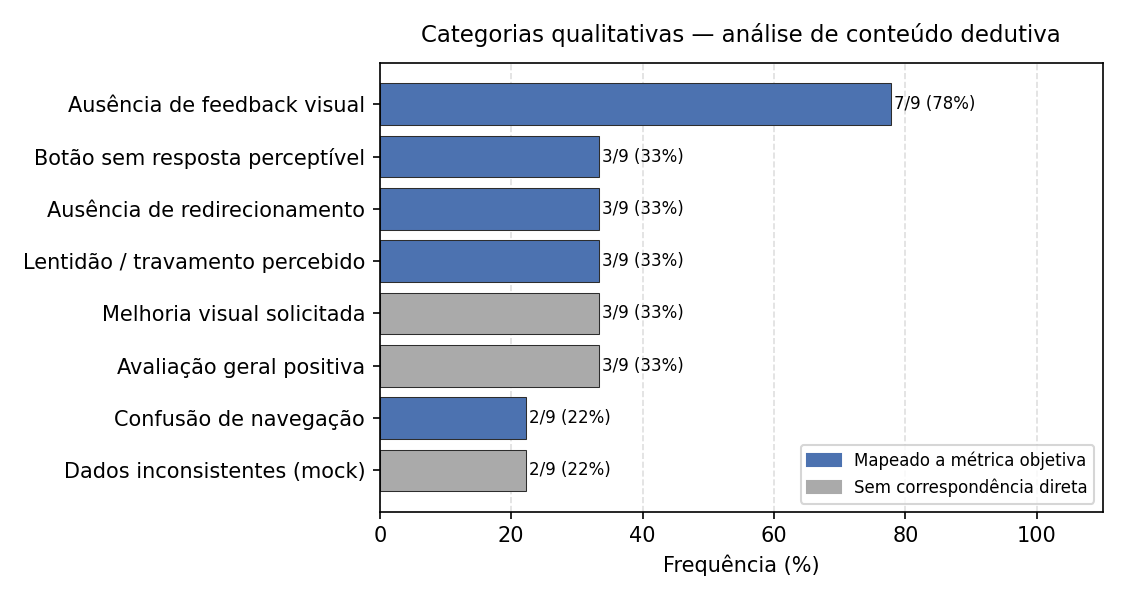
\includegraphics[width=0.98\linewidth]{plots/qualitative_themes_bar.png}
  \caption{Frequência das categorias qualitativas ($N = 9$). Barras em azul indicam categorias com correspondência direta a métrica objetiva do instrumento; cinza indica categorias sem correspondência instrumental.}
  \label{fig:temas}
\end{figure}

\begin{table}[htbp]
  \centering
  \caption{Frequência de temas nas respostas qualitativas ($N = 9$ participantes)}
  \begin{tabular}{p{4.5cm} r r p{4.5cm}}
    \toprule
    \textbf{Tema} & \textbf{N} & \textbf{\%} & \textbf{Relação com métrica objetiva} \\
    \midrule
    Ausência de \textit{feedback} visual & 7 & 78\% & \textit{dead clicks} e hesitações longas \\
    Botão sem resposta perceptível       & 3 & 33\% & \textit{dead clicks} $> 0$ \\
    Ausência de redirecionamento         & 3 & 33\% & hesitações longas pós-ação \\
    Lentidão / travamento percebido     & 3 & 33\% & duração elevada de fluxo \\
    Melhoria visual solicitada           & 3 & 33\% & -- \\
    Avaliação geral positiva             & 3 & 33\% & -- \\
    Confusão de navegação                & 2 & 22\% & duração elevada de fluxo \\
    Dados inconsistentes (mock)          & 2 & 22\% & -- (limitação da plataforma) \\
    \bottomrule
  \end{tabular}
\end{table}

O tema mais prevalente --- ausência de \textit{feedback} visual (78\%) --- mapeia diretamente os mecanismos de captura do instrumento. O participante P07 descreveu com precisão o fenômeno detectado automaticamente: \textit{``Ao clicar em `Salvar', fiquei esperando um retorno. Como não houve, cliquei várias vezes, entendendo que não havia funcionado anteriormente.''} De modo convergente, P08 relatou: \textit{``eu pensei que tinha travado a aplicação pois demorou e não mostrou algo diferente na tela''}. Esta triangulação confirma que os \textit{dead clicks} capturados pelo instrumento correspondem a comportamentos que os próprios usuários reconhecem e verbalizam espontaneamente.

\begin{figure}[htbp]
  \centering
  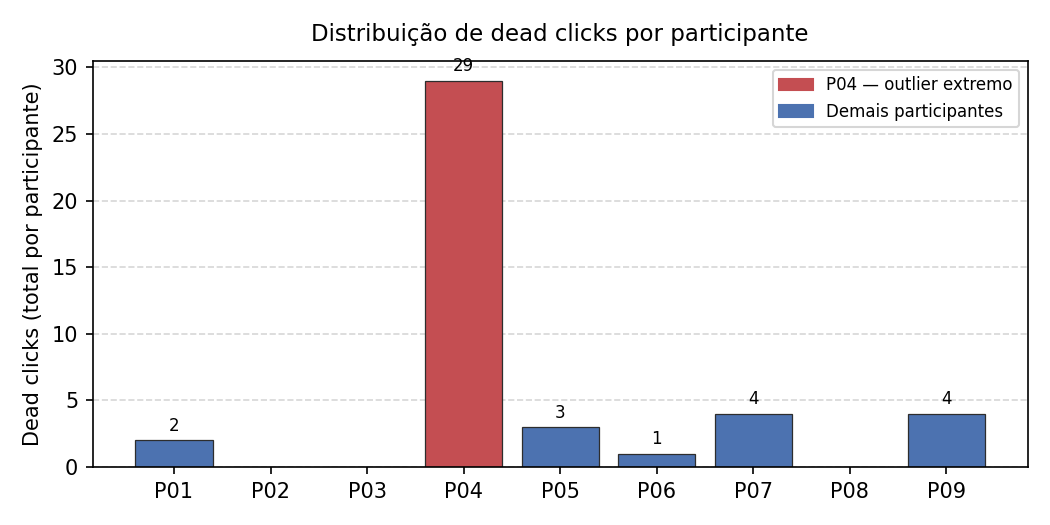
\includegraphics[width=0.92\linewidth]{plots/dead_clicks_by_participant.png}
  \caption{Distribuição de \textit{dead clicks} por participante. P04 constitui o \textit{outlier} extremo (29 eventos), com convergência nos dados subjetivos (UEQ-S pragmático $= -0{,}25$) e qualitativos (relato de botões sem resposta). Colorido em vermelho para distincção visual.}
  \label{fig:deadclicks}
\end{figure}

\subsection{Correlação de Spearman e Análise de Poder}

A correlação entre o \textit{FrictionScore} de sessão (composto por \textit{dead clicks}, hesitações e duração, normalizados por min-max, conforme descrito na Seção 4.1) e a qualidade pragmática UEQ-S resultou em $\rho = +0{,}13$ ($p \approx 0{,}73$, $N = 9$); para a escala hedônica, $\rho = -0{,}24$ ($p \approx 0{,}51$). Nenhuma correlação atingiu significância estatística. A direção negativa para a escala hedônica é teoricamente esperada: maior atrito comportamental deveria se associar a menor percepção de qualidade hedônica, uma vez que episódios de frustração pragmática contaminam a avaliação holística da experiência [Hassenzahl 2003].

Este resultado é esperado e metodologicamente previsível. A análise de poder \textit{a priori} --- via transformação Fisher-Z com $|\rho| = 0{,}5$, $\alpha = 0{,}05$ e poder $= 0{,}80$ --- indica que o estudo necessitaria de $N \geq 30$ participantes para resultados confirmatórios. Com $N = 9$, o Spearman opera como análise exploratória.

Ainda assim, o participante P04 --- o único com UEQ-S pragmático negativo ($-0{,}25$) --- apresentou o maior FrictionScore de sessão (70,76), com 29 \textit{dead clicks} e 20 hesitações longas. Seu relato qualitativo confirmou: \textit{``Os botões não funcionam, demoram a responder, não reencaminha para o feed''}. Esse caso demonstra que, em cenários de fricção grave, o instrumento e o autorrelato convergem de forma inequívoca.

\begin{figure}[htbp]
  \centering
  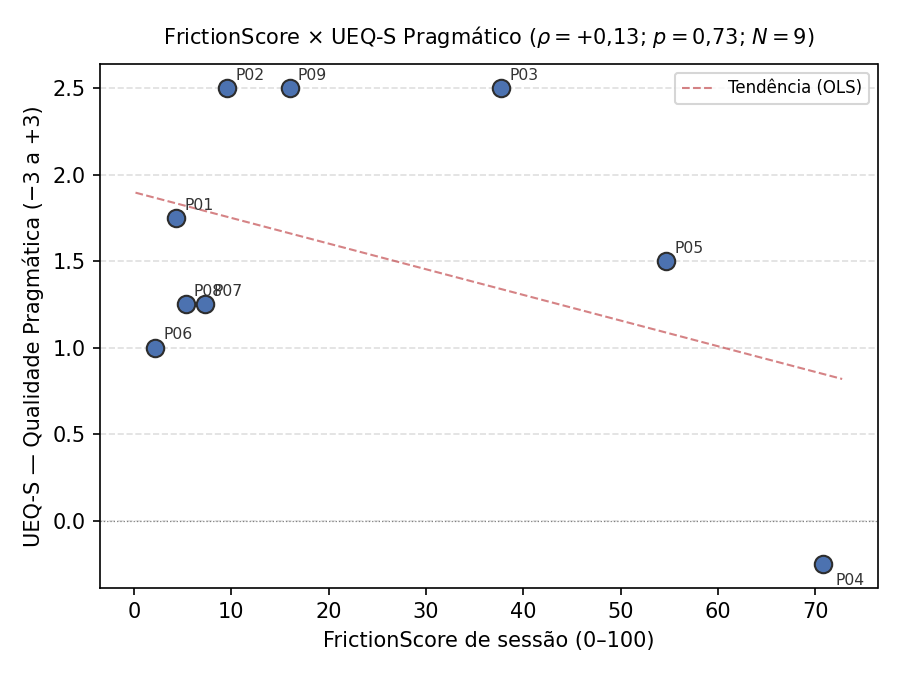
\includegraphics[width=0.85\linewidth]{plots/ueqs_scatter.png}
  \caption{\textit{FrictionScore} de sessão \textit{versus} qualidade pragmática UEQ-S por participante ($N = 9$). A linha tracejada representa a tendência OLS. A direção positiva de $\rho$ e a dispersão ampla ilustram o sub-dimensionamento estatístico ($N < 30$).}
  \label{fig:scatter}
\end{figure}

\subsection{Divergência Quali-Quanti e seus Significados}

Dois participantes apresentaram métricas objetivas elevadas combinadas a avaliações UEQ-S positivas: P03 (15 hesitações longas, duração de 1011 s) e P05 (44 hesitações longas). Esse padrão é consistente com dois fenômenos documentados na literatura de QoE. Primeiro, a \textit{Peak-End Rule} [Kahneman et al. 1993]: avaliações subjetivas de experiências são dominadas pelo pico emocional e pelo desfecho, não pela integração de todos os momentos. Quando a tarefa foi concluída com sucesso, episódios de espera intermediários tendem a ser subestimados no relato post-hoc. Segundo, o efeito de teto (\textit{ceiling effect}) do UEQ-S na versão curta: com apenas 4 itens pragmáticos e escala $-3$ a $+3$, o instrumento não discrimina diferenças dentro da faixa positiva [Möller et al. 2011, Sauro e Lewis 2012].

Esta divergência não enfraquece o estudo: pelo contrário, ela articula o argumento central em favor da medição comportamental automatizada. O instrumento captura atrito \textit{in situ} e de forma contínua, enquanto escalas subjetivas de aplicação única e poucos itens são estruturalmente limitadas para discernir fricções pontuais que o usuário supera e posteriormente racionaliza como aceitáveis.

\section{Conclusões e Trabalhos Futuros}

Este trabalho apresentou e validou um instrumento de medição automatizada de QoE baseado em Playwright, posicionado como auditor passivo de interações reais em um estudo controlado de métodos mistos. Os principais achados são:

\begin{itemize}
    \item \textbf{Validade de construto confirmada por triangulação:} 78\% dos participantes reportaram espontaneamente ausência de \textit{feedback} visual, o fenômeno primário capturado pela detecção de \textit{dead clicks} do instrumento;
    \item \textbf{Prova de conceito em caso extremo:} O participante com maior FrictionScore objetivo (70,76) foi o único com UEQ-S pragmático negativo e descreveu explicitamente os mesmos comportamentos capturados pelo instrumento;
    \item \textbf{Limitação metodológica identificada e quantificada:} Hesitações longas, quando analisadas isoladamente, são ambíguas (leitura vs. desorientação); a triangulação com \textit{dead clicks} e o qualitativo resolve a ambiguidade, mas exige coleta de múltiplos sinais. O Spearman requer $N \geq 30$ para resultados confirmatórios;
    \item \textbf{Limitação do instrumento subjetivo:} O efeito de teto do UEQ-S na versão curta limita a discriminação dentro da faixa positiva, favorecendo a complementaridade com métricas objetivas.
\end{itemize}

Como trabalhos futuros, propõe-se: (i) ampliar a amostra para $N \geq 30$ para análises confirmatórias; (ii) incorporar classificação semântica de hesitações (cognitiva vs. fricção) via análise de \textit{rawEvents}; (iii) instrumentalizar a medição real de requisições HTTP redundantes para quantificar diretamente o desperdício computacional associado a cada evento de \textit{dead click}.

% ==========================================
% REFERÊNCIAS
% ==========================================
\bibliographystyle{sbc}

\begin{thebibliography}{99}

\bibitem{sbsi2013}
[Autores SBSI 2013] (2013) ``Um estudo de caso sobre a avaliação energética de
software como uma contribuição à Computação Verde'', In: \textit{Anais do
Simpósio Brasileiro de Sistemas de Informação (SBSI 2013)}, SBC.

\bibitem{wsis}
[Autores WSIS] (Ano) ``Green IT: Sustainability as a Competitive Factor in the
IT Market'', In: \textit{Workshop de Sistemas de Informação (WSIS)}, SBC.

\bibitem{banaouas2019}
Banaouas, A. (2019) ``Automation of Heuristic-based Usability Inspection using
GUI Event Sequencing'', TU Wien.

\bibitem{bardin1977}
Bardin, L. (1977) \textit{L'Analyse de Contenu}, Presses Universitaires de
France, Paris.

\bibitem{hassenzahl2003}
Hassenzahl, M. (2003) ``The Thing and I: Understanding the Relationship Between
User and Product'', In: Blythe, M.~A., Overbeeke, K., Monk, A.~F., Wright,
P.~C. (Eds.), \textit{Funology: From Usability to Enjoyment}, Kluwer Academic
Publishers, pp.~31--42.

\bibitem{garcia2023}
Garcia, L.~A., Morandini, M., and Oliveira Jr, E. (2023) ``Uma Proposta para
Automatização de Avaliação de Usabilidade/UX'', In: \textit{Anais da VII
Escola Regional de Engenharia de Software (ERES 2023)}, SBC.

\bibitem{grigis2024}
Grigis, A. and De Angeli, A. (2024) ``Inductive analysis for UX research'',
In: \textit{Proceedings of the ACM CHI Conference}.

\bibitem{kahneman1993}
Kahneman, D., Fredrickson, B.~L., Schreiber, C.~A., and Redelmeier, D.~A.
(1993) ``When More Pain Is Preferred to Less: Adding a Better End'',
\textit{Psychological Science}, 4(6):401--405.

\bibitem{keshvadi2020}
Keshvadi, S. and Williamson, C. (2020) ``MoVIE: A Measurement Tool for Mobile
Video Streaming on Smartphones'', In: \textit{Proceedings of the ACM/SPEC
International Conference on Performance Engineering (ICPE)}, ACM.

\bibitem{leppanen2024}
Leppänen, J. (2024) ``Forestry machine user interface testing'', Master's
thesis, LAB University of Applied Sciences.

\bibitem{molich1990}
Molich, R. and Nielsen, J. (1990) ``Improving a human-computer dialogue'',
\textit{Communications of the ACM}, 33(3):338--348.

\bibitem{moller2011}
Möller, S., Engelbrecht, K.-P., Kühnel, C., Wechsung, I., and Weiss, B. (2011)
``A Taxonomic Approach to Evaluate and Compare Quality of Experience'', In:
\textit{Proceedings of Eighth International Workshop on Quality of Multimedia
Experience (QoMEX)}, IEEE.

\bibitem{nielsen1994}
Nielsen, J. (1994) ``Enhancing the explanatory power of usability heuristics'',
In: \textit{Proceedings of the SIGCHI conference on Human Factors in Computing
Systems}, pp.~152--158.

\bibitem{oyedeji2019}
Oyedeji, S., Naqvi, B., Penzenstadler, B., Adisa, M.~O., and Abdulkareem,
M. (2019) ``The Interplay between Usability, Sustainability and Green Aspects:
A Design Case Study from a Developing Country'', In: \textit{Proceedings of
the 6th International Conference on ICT for Sustainability (ICT4S)}.

\bibitem{rani2024}
Rani, P., Zellweger, J., Kousadianos, V., Cruz, L., Kehrer, T., and
Bacchelli, A. (2024) ``Energy Patterns for Web: An Exploratory Study'', In:
\textit{Proceedings -- 2024 ACM/IEEE 46th International Conference on Software
Engineering (ICSE-SEIS 2024)}, IEEE.

\bibitem{rousi2019}
Rousi, R. (2019) ``From empty signifiers to the Chinese room: A critique of
automated user experience'', In: \textit{IFIP Conference on Human-Computer
Interaction}, Springer.

\bibitem{savoldi2018}
Savoldi, G. e Oliveira, R.~A.~P. (2018) ``Estudo e aplicação da ferramenta
sikuli para auxílio em testes funcionais e de usabilidade por meio da
automação por imagem'', In: \textit{Anais da II Escola Regional de Engenharia
de Software (ERES 2018)}, SBC.

\bibitem{sauro2012}
Sauro, J. and Lewis, J.~R. (2012) \textit{Quantifying the User Experience:
Practical Statistics for User Research}, Elsevier, Amsterdam.

\bibitem{searle1982}
Searle, J.~R. (1982) ``The Chinese room revisited'',
\textit{Behavioral and Brain Sciences}.

\bibitem{teixeira2025}
Teixeira, R.~S.~V. and Fook, K.~D. (2025) ``Catálogo de Requisitos para
Software Sustentável'', In: \textit{Anais Estendidos do Simpósio Brasileiro de
Qualidade de Software (SBQS 2025)}, SBC.

\end{thebibliography}

\end{document}